\chapter{Metodologías a usar en el proyecto}
\label{ch:metodologias}
En este capítulo se explicaran las diferentes metodologías que serán utilizadas para desarrollar el proyecto, estas incluyen metodologías de desarrollo ágil, diseño centrado en el usuario y el proceso de desarrollo de videojuegos.

\section{Metodologías de desarrollo ágil}
El desarrollo del proyecto se llevará a cabo utilizando metodologías de desarrollo ágil, estas surgen a partir del Manifiesto Ágil \cite{beck}. Más concretamente se utilizarán elementos de Scrum, que se basa en un desarrollo iterativo, en el que el producto se irá construyendo por etapas, y será testeado en cada una de dichas etapas, permitiendo así una temprana solución de errores, y añadiendo también un valor extra al producto al haber sido testeado varias veces durante el desarrollo por usuarios reales. El desarrollo ágil también permitirá una mas sencilla organización del proyecto, en la que a partir de un plan de entregas inicial se organizan iteraciones para ir cumpliendo los objetivos de estas entregas.\\

\newpage

En la Figura \ref{figura-agile} se puede observar un esquema del desarrollo por iteraciones:

\begin{figure}[h]
  \centering
  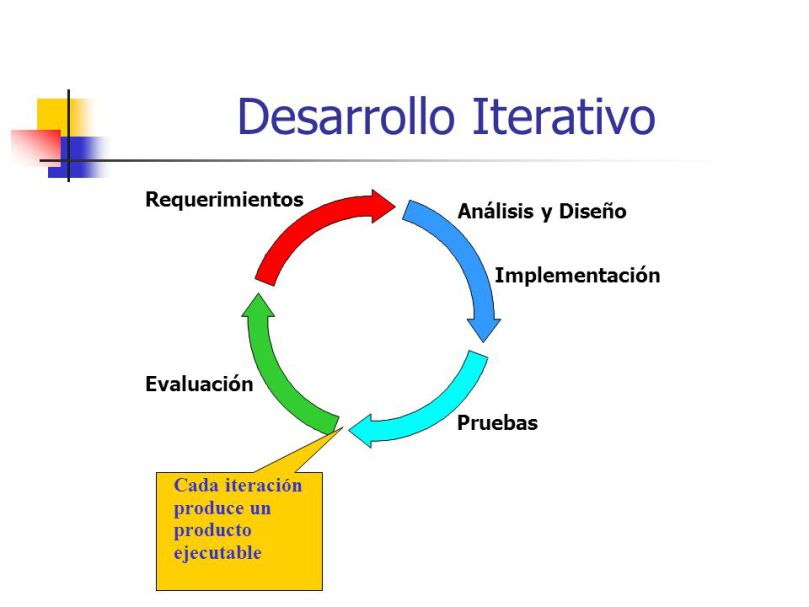
\includegraphics[scale=0.45]{agile}
  \caption{Imagen que muestra un proceso de desarrollo iterativo.\protect\footnotemark}
  \label{figura-agile}
\end{figure}

\footnotetext{Yuukiter, {\em Desarrollo de Software Iterativo}, RUP, Recuperado de \\
\url{https://rupnoobs.wordpress.com/2016/03/10/desarrollo-de-software-iterativo/}, (11 de marzo de 2016).}

El primer elemento relevante que se utilizará en el desarrollo son las historias de usuario, que nos permitirán establecer unos requisitos iniciales para la aplicación de una forma sencilla y completa. A estas historias de usuario se les asignará una entrega para la que la historia deberá estar completa y una iteración en la que se lleva a cabo, de forma que se obtiene de una forma organizada cuales son las partes del producto que tienen que estar listas para cada entrega.\\

Dentro de cada entrega puede existir una o varias iteraciones, estas se planificarán al inicio cuando se define dicha iteración, y contendrá las tareas a realizar en cada iteración, que suelen ser historias de usuario, pero que también pueden incluir otras tareas de documentación o tareas necesarias para el desarrollo, que no necesariamente son una historia de usuario, como por ejemplo, obtener los modelos 3D que serán necesarios para el juego.\\

Por otro lado se realizarán entregas, que quedan detalladas en el plan de entregas creado al inicio del proyecto. Al final de cada entrega se obtendrá un producto, que será testeado tanto por el desarrollador como por los usuarios.

\subsection{Diseño centrado en el usuario}
Uno de los principios del desarrollo ágil es la satisfacción del usuario, por tanto, el desarrollo de este proyecto también esta enfocado en el diseño centrado en el usuario \cite{sanchez}, de forma que, gracias a una organización por iteraciones y con entregas, se obtenga una retroalimentación por parte del usuario en cada entrega.\\

El proceso por iteraciones del diseño centrado en el usuario que se puede observar en la Figura \ref{figura-iteraciones}, se integra con las entregas iniciales que es cuando se esta llevando a cabo el diseño, y por tanto, donde quedará definido este, las etapas de una iteración para el diseño centrado en el usuario son diferentes a las de una iteración del desarrollo, ya que estas específicamente se centran en el diseño.

\begin{figure}[h]
  \centering
  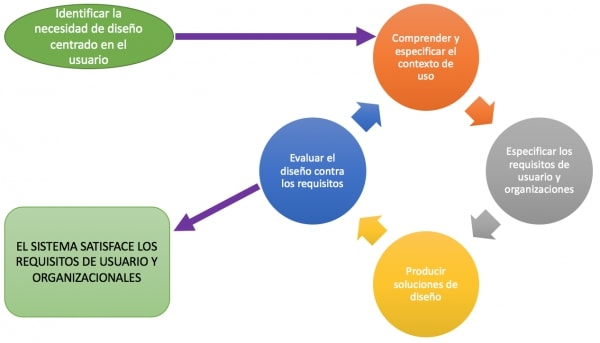
\includegraphics[scale=0.6]{iteraciones}
  \caption{Imagen que muestra un proceso de desarrollo iterativo centrado en el usuario.\protect\footnotemark}
  \label{figura-iteraciones}
\end{figure}

\footnotetext{Alfredo, {\em ¡Diseña centrándote en el usuario!}, Time of Software, Recuperado de \\
\url{http://timeofsoftware.com/disena-centrandote-en-el-usuario/}, (16 de enero de 2017).}

\newpage

Estas etapas son:
\begin{itemize}
  \item Se especifica el contexto de uso para entender la situación del usuario.
  \item Basado en dicho contexto se establecen los requisitos.
  \item Una vez obtenidos los requisitos se hacen las soluciones de diseño.
  \item Finalmente se evalúa el producto probándolo con el usuario.
\end{itemize}

Las evaluaciones del diseño al final de cada iteración coinciden con las entregas iniciales, que suponen una fecha en la que se presenta un producto al usuario, y se realizan pruebas sobre dicho producto, de forma que el usuario esta utilizando el producto, lo que permite una realimentación por parte del usuario de forma periódica, para detectar fallos o posibles mejoras sobre el diseño a tiempo, y solventarlos, de manera que el producto final, sea lo mas sencillo de utilizar por el usuario, este proceso a su vez, esta incrementando el valor del producto, preparándolo para que en el momento que se lance al mercado, los fallos sean mínimos y la experiencia del usuario final sea excelente.\\

Por tanto, este proceso es beneficioso para el usuario, ya que todo el desarrollo esta centrado en que el producto le ofrezca una buena experiencia, ya que al fin y al cabo, es el usuario el que está en contacto con el producto a diario. Y todo esto es posible ya que todo el proceso de desarrollo está orientado al usuario y su experiencia utilizando el producto.

\section{Desarrollo de videojuegos}
Un modelo bastante utilizado en el desarrollo de videojuegos lo podemos encontrar en \cite{pereira}, este divide dicho desarrollo en tres etapas, como se puede ver en la Figura \ref{figura-pre-pro-post}, las etapas son:

\begin{itemize}
  \item \textbf{Pre-producción}: En esta etapa se realiza una definición del juego, con sus característica mas importantes, y como resultado se obtiene una versión inicial el GDD, que es el documento que contiene el diseño del videojuego.
  \item \textbf{Producción}: En esta etapa se realizan varias tareas distintas:

  \begin{itemize}
    \item \textbf{Diseño artístico}: En esta etapa se desarrollan los conceptos mas relacionados con la apariencia del juego, como pueden ser la historia, sonidos, interfaz y gráficos.
    \item \textbf{Diseño mecánico}: En esta etapa se crea la mecánica del juego, es decir, como va a ser la interacción del jugador con el juego y como va a funcionar la inteligencia artificial del juego.
    \item \textbf{Diseño técnico}: En esta etapa se desarrolla la dinámica interna del juego, que incluye diagramas de clase, diagramas de secuencia, los estados en los que se encontrará el juego en diferentes puntos a nivel de software, etc.
    \item \textbf{Implementación}: En esta etapa todas las partes que se han ido desarrollando por separado se unen, de forma que encajen perfectamente como una en el juego.
    \item \textbf{Pruebas alpha}: En esta etapa se hacen pruebas sobre un producto ya terminado, para verificar que el proyecto ya está convertido en producto y se puede poner dicho producto en el mercado.
    \item \textbf{Pruebas beta}: En esta etapa se hacen pruebas para intentar quitar todos los defectos posibles que el juego pueda tener, y que cuando el producto salga al mercado esté en perfecto estado. También se comprueban aspectos legales para asegurar que no habrá problemas con las normativas de los distintos países en los que se publicará.
    \item \textbf{Gold master}: Es la copia del juego definitiva una vez finalizado el proyecto.
  \end{itemize}

  \item \textbf{Post-producción}: Esta etapa ocurre una vez el juego ya está en el mercado, aquí se hace un seguimiento de como esta funcionando el producto, si hay que cambiar de estrategia o buscar formas de explotarlo más.

\end{itemize}

\begin{figure}[h]
  \centering
  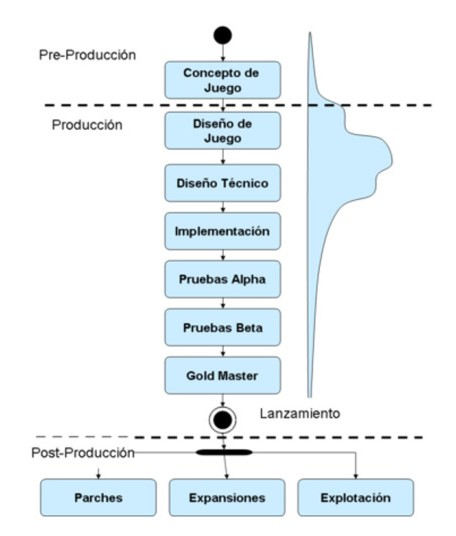
\includegraphics[scale=0.6]{pre-pro-post}
  \caption{Imagen que muestra el proceso de desarrollo de un videojuego separado en las etapas de pre-producción, producción y post-producción.\protect\footnotemark}
  \label{figura-pre-pro-post}
\end{figure}

\footnotetext{Pereira, A. M. M., {\em El proceso productivo del videojuego: fases de producción/The production process of the game: production phases}. Historia y Comunicación Social, 19, 791-805. (2014).}

\newpage

Como se puede ver en este método de desarrollo de videojuegos, el documento de diseño de videojuegos es un elemento central.\\

El GDD es la base del desarrollo del videojuego, ya que este contiene toda la información acerca de como tiene que ser cada aspecto de este, generalmente contiene los siguientes elementos entre otros:

\begin{itemize}
  \item Género
  \item Jugadores
  \item Historia
  \item Interfaz de usuario
  \item Objetivos
  \item Reglas
  \item Etc
\end{itemize}

Como se puede comprobar por los elementos que se encuentran en el GDD, este documento contiene toda la información sobre el juego que es relevante para la implementación, por lo que es fundamental en el desarrollo, para una vez estemos implementando adherirnos a la lo descrito en el GDD y consultar cualquier duda en él.

\section{Conclusiones}
Todas estas metodologías se utilizarán en conjunto en este proyecto, y serán aplicadas de la siguiente forma:

\begin{itemize}
  \item Primero de todo se realizarán las historias de usuario, de esta manera obtendremos los requisitos del juego.
  \item Se realizará el plan de entregas, de forma que cada una de dichas entregas tiene un objetivo a cumplir, este objetivo es un prototipo con ciertas características completadas.
  \item Se realizarán las iteraciones que forman cada entrega dentro del plan de entregas, estas tendrán una duración de una semana, y tendrán unas tareas asignadas, dichas tareas pueden ser historias de usuario y tienen que ser completadas en el objetivo de tiempo para así llegar a tiempo a la entrega programada. Las iteraciones sirven para dividir las tareas en periodos mas cortos de tiempo, y además para añadir tareas que no forman parte de la entrega pero que son necesarias para el desarrollo.
  \item Se realizarán pruebas heurísticas y de usabilidad en cada entrega, de forma que se obtenga información por parte de los usuarios del estado del producto, de los errores que tiene y los aspectos a mejorar.
  \item Se comenzará a desarrollar el documento de diseño de videojuegos en las primeras iteraciones, para establecer los conceptos iniciales del juego, y se modificará durante todo el proceso de desarrollo, ya que el GDD es un documento vivo que va modificándose en función de como avanza el desarrollo y las pruebas con usuarios.
\end{itemize}
